\section{Third strategy - Daltonism may help}

As with previous strategies, we order the vertices according to $col_{2}(G)$.
We would like to draw your attention to the fact that we no longer use the loose backward neighbors, just the backward neighbors, i.e. neighbors with a lower index in the order.

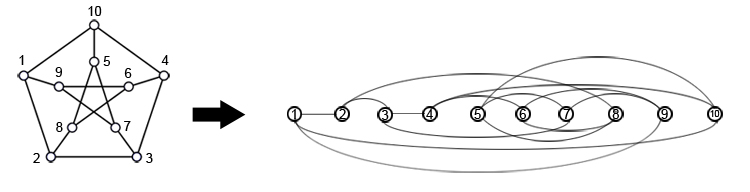
\includegraphics[width=13cm]{IntroOrder.jpg}

In this case, we use a rather simple activation strategy.
When Bob colors a vertex $v$, Alice begins by activating the vertex $v$, then she checks its backward neighbors.
$x$ is the backward neighbor of $v$ having the lowest index in the order.
If $x$ is colored, we turn to the next backward neighbor of $v$. If $x$ is activated, then it is in danger and we give it a color. If $x$ is not activated, then we activate it and we check its backward neighbors. If x has no unshaded backward neighbor, then we color $x$.
In the case where the vertex v (colored by Bob) has no unshaded backward neighbor, then we color the unshaded vertex having the lowest index in the order previously calculated.


According to this strategy, each graph satisfies $\chi_{g}(G) \leq 3 \times col_{2}(G) - 1$.

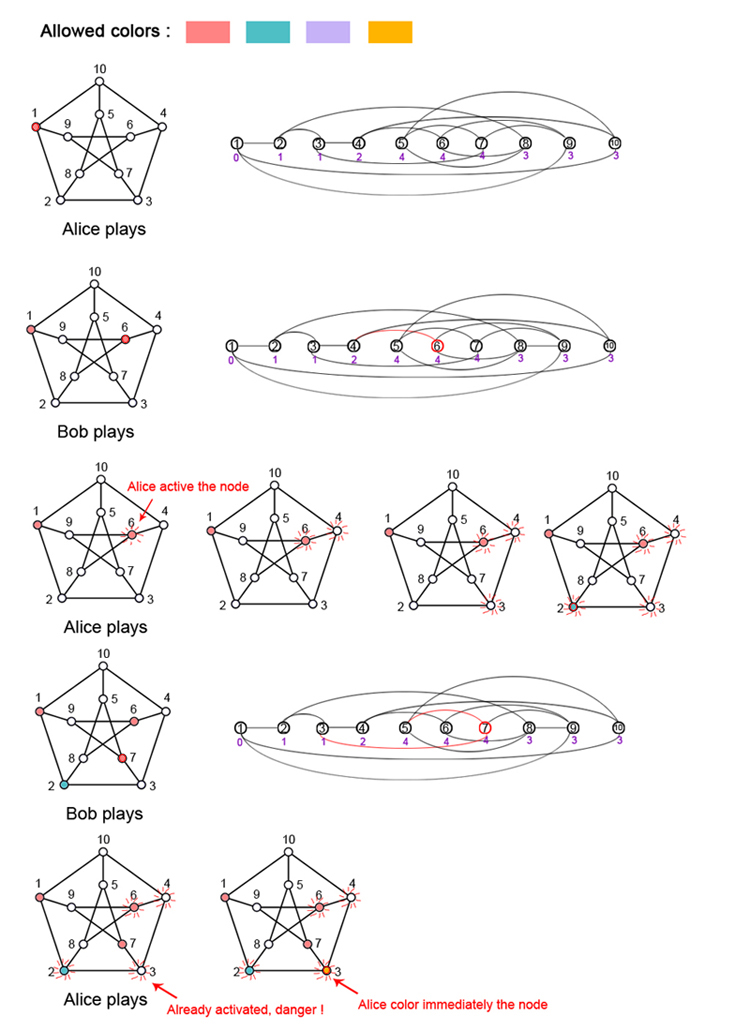
\includegraphics[width=15cm]{gameS3.jpg}